\documentclass{article}%
\usepackage[T1]{fontenc}%
\usepackage[utf8]{inputenc}%
\usepackage{lmodern}%
\usepackage{textcomp}%
\usepackage{lastpage}%
\usepackage[head=40pt,margin=0.5in,bottom=0.6in]{geometry}%
\usepackage{graphicx}%
%
\title{\textbf{Vecinos en los Ruices denuncian insalubridad ante falta de recolección de basura}}%
\author{NOTA DE PRENSA}%
\date{02/10/2018}%
%
\begin{document}%
\normalsize%
\maketitle%
\textbf{URL: }%
http://www.eluniversal.com/caracas/22188/vecinos{-}en{-}los{-}ruices{-}denuncian{-}insalubridad{-}ante{-}falta{-}de{-}recoleccion{-}de{-}basura\newline%
%
\textbf{Periodico: }%
EU, %
ID: %
22188, %
Seccion: %
caracas\newline%
%
\textbf{Palabras Claves: }%
NO\_TIENE\newline%
%
\textbf{Derecho: }%
3.2%
, Otros Derechos: %
NO\_TIENE%
, Sub Derechos: %
3.2.1%
\newline%
%
\textbf{EP: }%
NO\newline%
\newline%
%
\textbf{\textit{Manifestaron que pueden pasar varios días sin que vayan los camiones recolectores por lo que las bolsas de basura se acumula progresivamente en las calles y cuartos de desperdicios de los edificios.}}%
\newline%
\newline%
%
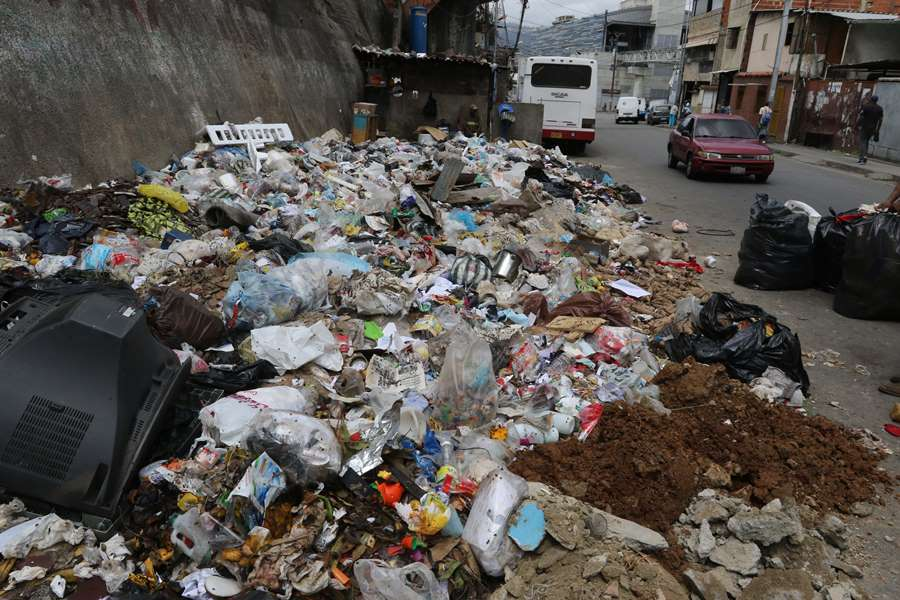
\includegraphics[width=300px]{172.JPG}%
\newline%
%
Caracas.{-} Vecinos de Los Ruices denunciaron la situación sanitaria que padecen producto de la acumulación de basura en las aceras, calles y avenidas, por ineficacia de la Alcaldía del municipio Sucre y la falla en el saneamiento de quebradas, poda de árboles y fumigación en esa comunidad.%
\newline%
%
La reunión organizada por la asociación de vecinos ASODONBOSCO, en una asamblea realizada en el Parque Simón Rodríguez, con el apoyo del concejal Manfredo González, de la Comisión de Ecología y Ambiente de Sucre y Caracas Ciudad Plural, se convocó para que los representantes de las juntas de vecinos, consejos comunales y habitantes en general de la zona realizaran sus reclamos al presidente del Instituto Autónomo de Protección y Saneamiento Ambiental de Sucre (IMAPSAS), José Vicente Rangel Seijó, quien asistió acompañado de autoridades de ese ente municipal para recibir las exigencias.%
\newline%
%
Los vecinos manifestaron que pueden pasar varios días sin que vayan los camiones recolectores  por lo que las bolsas de basura se acumula progresivamente en las calles y cuartos de desperdicios de los edificios y casas, y esto aunado al aumento de grupos de personas que hurgan entre los basureros y bolsas en buscan de comida y esparcen los desperdicios por las aceras incrementan los riesgos de salubridad.%
\newline%
%
Griselda Borges, residente del edificio Bambusal, comentó que se han presentado casos de Zica entre sus vecinos debido a la proliferación de zancudos consecuencia de la ausencia de mantenimiento de la quebrada aledaña y la falta de fumigación en las residencias por parte de la Alcaldía desde hace mucho tiempo.%
\newline%
%
La representante del Consejo Comunal Los Ruices Socialista, cuestionó que las autoridades, no asuman la denuncia con relación a una alcantarilla de aguas negras  cerca de las Residencias San Francisco, que desborda sus aguas fétidas por la calle generando un peligroso foco de mosquitos y moscas verdes.%
\newline%
%
El concejal Manfredo González, también coordinador de Caracas Ciudad Plural, propuso a la comunidad una alternativa de reciclaje para reducir el volumen de basura que se entrega a la operadora de recolección de la Alcaldía y que además influye directamente en la disminución de costos para las comunidades al utilizarse menos bolsas de basura.%
\newline%
%
El proyecto es una alianza entre Caracas Ciudad Plural y la Empresa Multirecicla, que se ha aplicado exitosamente en el Municipio Baruta y varias localidades, el cual consiste en disponer unos contenedores debidamente identificados en edificios, casas o establecimientos comerciales, en los que se depositan únicamente materiales para reciclar (plástico, vidrio, cartón y envases TetraPak) posteriormente Multirecicla, de manera gratuita, se encarga de la recolección, traslado, almacenamiento, separación, procesamiento y disposición del desecho para ubicarlo con las empresas de producción de materia prima, de esta manera contribuimos a reducir nuestro impacto en el planeta, a cuidar el ambiente y a crear una sociedad sostenible.%
\newline%
%
\end{document}